\section{最优解的变化}
\label{sec:sens-solution}

最优值是一个数，最优解是一个向量，后者需要更多的结构才能求导。这就需要回答：选定一个解之后，它随参数怎样移动？办法是把这个解满足的最优性条件看成一组方程，方程里既有原变量和乘子，也有参数，然后像解隐函数那样求局部导数。

\paragraph{隐函数定理的回顾}
所用的工具是隐函数定理：设$\bm{F}(\bm{z},\bm{\theta})$连续可微，$\bm{F}(\bm{z}_0,\bm{\theta}_0)=\bm{0}$，方阵$\bm{D}_{\bm{z}}\bm{F}(\bm{z}_0,\bm{\theta}_0)$可逆。则在$\bm{\theta}_0$附近有唯一的连续可微映射$\bm{z}(\bm{\theta})$，使$\bm{z}(\bm{\theta}_0)=\bm{z}_0$，且在$(\bm{z}_0,\bm{\theta}_0)$的某个邻域内方程的解全部落在这条曲线上。它的导数满足线性方程
\[
 \bm{D}_{\bm{z}}\bm{F}\cdot\bm{D}\bm{z}=-\bm{D}_{\bm{\theta}}\bm{F}.
\]
定理的陈述与证明可参考\BookChapterRef{chap:implicit-inverse-functions}{卷二第22章“隐函数与反函数”}。

用它研究极小点时要多一步检查，因为隐函数定理只管方程。例如$f(x,\theta)=-x^2/2+\theta x$的驻点方程是$-x+\theta=0$，导数$-1$可逆，隐函数定理给出光滑分支$x(\theta)=\theta$，而这条分支上全是极大点。所以下面每个定理都分成两部分：方程有光滑解，以及这个解确实是极小点。

\subsection{无约束极小解}
\label{sec:sens-unconstrained}

\paragraph{碗的曲率决定碗底移动的距离}
无约束时，$\bm{x}^\star$是碗底，满足$\nabla_{\bm{x}}f=\bm{0}$。参数一变，梯度在原来的位置上不再为零，碗底要移动到新的梯度零点。线性近似告诉我们移动多少：
\[
 \nabla^2_{\bm{x}\bm{x}}f\cdot\Delta\bm{x}+\nabla^2_{\bm{x}\bm{\theta}}f\cdot\Delta\bm{\theta}\approx\bm{0}.
\]
曲率大的方向，碗壁陡，碗底只需移动一点就能抵消参数带来的梯度变化；曲率小的方向，碗底要移动很远。

\begin{theorem}[无约束极小解的导数]
\label{thm:sens-unconstrained}
设$f$在$(\bm{x}_0,\bm{\theta}_0)$的邻域内二阶连续可微，$\nabla_{\bm{x}}f(\bm{x}_0,\bm{\theta}_0)=\bm{0}$，$\nabla^2_{\bm{x}\bm{x}}f(\bm{x}_0,\bm{\theta}_0)\succ\bm{0}$。则存在$\bm{\theta}_0$的邻域和唯一的连续可微映射$\bm{x}(\cdot)$，使$\bm{x}(\bm{\theta}_0)=\bm{x}_0$，且邻域内的每个$\bm{x}(\bm{\theta})$都是$f(\cdot,\bm{\theta})$的严格局部极小点。Jacobian矩阵$\bm{D}_{\bm{x}}\in\mathbb{R}^{n\times q}$由线性方程
\begin{equation}
 \nabla^2_{\bm{x}\bm{x}}f\cdot\bm{D}_{\bm{x}}=-\nabla^2_{\bm{x}\bm{\theta}}f
 \label{eq:sens-unconstrained-derivative}
\end{equation}
确定，其中各导数都在$(\bm{x}(\bm{\theta}),\bm{\theta})$处取值。
\end{theorem}

\begin{proof}
令$\bm{F}=\nabla_{\bm{x}}f$。$f$二阶连续可微，所以$\bm{F}$连续可微。$\bm{D}_{\bm{x}}\bm{F}=\nabla^2_{\bm{x}\bm{x}}f$在基准点正定，因而可逆。隐函数定理给出连续可微的分支$\bm{x}(\bm{\theta})$，对恒等式$\bm{F}(\bm{x}(\bm{\theta}),\bm{\theta})=\bm{0}$求导就得到式~\eqref{eq:sens-unconstrained-derivative}。

再说明它是极小点。Hessian矩阵连续依赖于$(\bm{x},\bm{\theta})$，矩阵的最小特征值连续，所以$\bm{\theta}$靠近$\bm{\theta}_0$时，$\nabla^2_{\bm{x}\bm{x}}f(\bm{x}(\bm{\theta}),\bm{\theta})$仍然正定。驻点处Hessian正定，由第~\ref{chap:smooth-foundations}章的二阶充分条件，$\bm{x}(\bm{\theta})$是严格局部极小点。
\end{proof}

定理是局部的，Hessian正定只说明这条分支是局部极小，它不保证全局最优。正定性也不能减弱成可逆：上面驻点是极大点的例子中，Hessian可逆但负定。

\paragraph{例子：带二次惩罚的最小二乘}
取$\bm{A}$和$\bm{b}$如下，并用$\gamma>0$作正则系数：
\[
 \bm{A}=\begin{bmatrix}1&1\\1&0\end{bmatrix},\qquad
 \bm{b}=\begin{bmatrix}2\\0\end{bmatrix},\qquad
 f(\bm{x},\gamma)=\frac12\lVert\bm{A}\bm{x}-\bm{b}\rVert_2^2+\frac{\gamma}{2}\lVert\bm{x}\rVert_2^2.
\]
梯度为零的方程是$\bm{H}(\gamma)\bm{x}=\bm{A}^{\top}\bm{b}$，其中
\[
 \bm{H}(\gamma)=\bm{A}^{\top}\bm{A}+\gamma\bm{I}=\begin{bmatrix}2+\gamma&1\\1&1+\gamma\end{bmatrix},\qquad
 \bm{A}^{\top}\bm{b}=\begin{bmatrix}2\\2\end{bmatrix}.
\]

$\gamma>0$时$\bm{H}(\gamma)$正定，所以全局最优解存在且唯一，条件满足。在$\gamma=1$处，求$\bm{H}$的逆矩阵，得到
\[
 \bm{H}(1)=\begin{bmatrix}3&1\\1&2\end{bmatrix},\qquad
 \bm{H}(1)^{-1}=\frac15\begin{bmatrix}2&-1\\-1&3\end{bmatrix},\qquad
 \bm{x}(1)=\begin{bmatrix}2/5\\4/5\end{bmatrix}.
\]

梯度$\bm{H}(\gamma)\bm{x}-\bm{A}^{\top}\bm{b}$对$\gamma$的偏导数是$\bm{x}$本身。于是式~\eqref{eq:sens-unconstrained-derivative}给出
\[
 \bm{x}'(1)=-\bm{H}(1)^{-1}\bm{x}(1)=\begin{bmatrix}0\\-2/5\end{bmatrix}.
\]

$\gamma$增大时，解在这一点上只往$x_2$减小的方向移动，$x_1$的一阶变化恰好为零。显式解是
\[
 x_1(\gamma)=\frac{2\gamma}{1+3\gamma+\gamma^2},\qquad
 x_2(\gamma)=\frac{2+2\gamma}{1+3\gamma+\gamma^2},
\]
直接求导可以验证同一结果，$x_1(\gamma)$恰在$\gamma=1$达到最大。

\paragraph{局部导数与有限跳变}
一阶预测$\bm{x}(1)+(\gamma-1)\bm{x}'(1)$的可信范围是有限的。$\gamma=1.1$时，真解和预测分别是
\[
 \bm{x}(1.1)\approx(0.3993,\ 0.7623),\qquad
 \bm{x}(1)+0.1\,\bm{x}'(1)=(0.4,\ 0.76).
\]
两者很接近。$\gamma=3$时，真解是$(6/19,8/19)\approx(0.316,0.421)$，而预测是$(0.4,0)$，差得很远。图~\ref{fig:sens-ridge-path}显示了原因：解的路径是弯的，切线只在基准点附近贴着它。

\begin{BookInlineFigure}
 \centering
 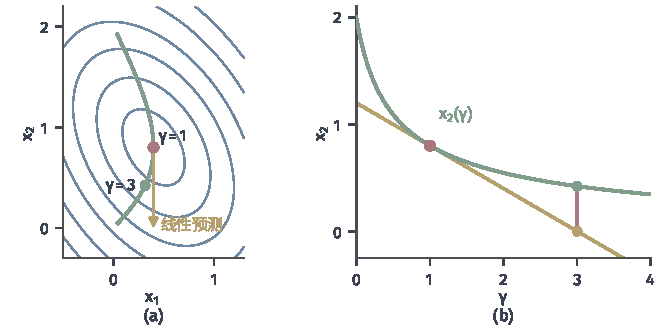
\includegraphics[width=112mm]{figures/05-optimization/06-constrained-optimization/matplotlib/sens-ridge-path/figure.pdf}
 \caption{带二次惩罚的最小二乘的解随$\gamma$的移动。(a)~蓝线是$\gamma=1$的目标等高线，绿色曲线是解的路径，红点是$\bm{x}(1)$，绿点是$\bm{x}(3)$，黄色箭头是导数给出的线性预测。(b)~$x_2(\gamma)$（绿线）与它在$\gamma=1$的切线（黄线），红色线段是$\gamma=3$处的预测误差。}
 \label{fig:sens-ridge-path}
\end{BookInlineFigure}

导数回答的是无穷小的变化。有限跳变需要另外的工具。下面的结论不需要解分支可微，对任意大小的参数差都成立。

\begin{theorem}[强凸情形的有限跳变界]
\label{thm:sens-finite-jump}
设对$\bm{\theta}\in\{\bm{\theta}_0,\bm{\theta}_1\}$，$f(\cdot,\bm{\theta})$在$\mathbb{R}^n$上可微，$\bm{x}_0$、$\bm{x}_1$分别是$f(\cdot,\bm{\theta}_0)$、$f(\cdot,\bm{\theta}_1)$的最小点，且$f(\cdot,\bm{\theta}_1)$是$\mu$强凸的。则
\begin{equation}
 \lVert\bm{x}_1-\bm{x}_0\rVert_2\leq\frac{1}{\mu}\bigl\lVert\nabla_{\bm{x}}f(\bm{x}_0,\bm{\theta}_1)-\nabla_{\bm{x}}f(\bm{x}_0,\bm{\theta}_0)\bigr\rVert_2.
 \label{eq:sens-finite-jump}
\end{equation}
\end{theorem}

\begin{proof}
强凸函数的梯度满足
\[
 \bigl\langle\nabla_{\bm{x}}f(\bm{x}_1,\bm{\theta}_1)-\nabla_{\bm{x}}f(\bm{x}_0,\bm{\theta}_1),\ \bm{x}_1-\bm{x}_0\bigr\rangle\geq\mu\lVert\bm{x}_1-\bm{x}_0\rVert_2^2.
\]
$\bm{x}_1$是$f(\cdot,\bm{\theta}_1)$的最小点，所以左端第一个梯度为零。$\bm{x}_0$是基准问题的最小点，零向量$\nabla_{\bm{x}}f(\bm{x}_0,\bm{\theta}_0)$可以加进去而不改变左端。于是
\[
 \mu\lVert\bm{x}_1-\bm{x}_0\rVert_2^2\leq\bigl\langle\nabla_{\bm{x}}f(\bm{x}_0,\bm{\theta}_0)-\nabla_{\bm{x}}f(\bm{x}_0,\bm{\theta}_1),\ \bm{x}_1-\bm{x}_0\bigr\rangle.
\]
用Cauchy--Schwarz不等式放大右端，再除以$\lVert\bm{x}_1-\bm{x}_0\rVert_2$（为零时结论直接成立），就得到式~\eqref{eq:sens-finite-jump}。
\end{proof}

式~\eqref{eq:sens-finite-jump}右端衡量“新目标在旧解处的梯度有多大”，$1/\mu$把这个梯度折算成距离，这与隐式导数中的逆Hessian起同样的作用。

在岭回归的例子里，$\gamma_0=1$，$\gamma_1=3$，新旧目标在$\bm{x}_0$处的梯度差是$(\gamma_1-\gamma_0)\bm{x}_0$，强凸常数是
\[
 \mu=3+\lambda_{\min}(\bm{A}^{\top}\bm{A})=3+\frac{3-\sqrt{5}}{2}.
\]
算出的上界和真实距离分别是
\[
 \frac{2\lVert\bm{x}_0\rVert_2}{\mu}\approx0.529,\qquad
 \lVert\bm{x}(3)-\bm{x}(1)\rVert_2\approx0.388.
\]
真实距离没有超过上界。

\paragraph{预测误差受三阶信息控制}
一阶预测的误差要看导数变化得多快。下面的情形最容易说清楚：参数以线性项进入目标。

\begin{theorem}[线性扰动下的预测误差]
\label{thm:sens-prediction-error}
设$\varphi:\mathbb{R}^n\to\mathbb{R}$二阶连续可微、$\mu$强凸，$\nabla^2\varphi$是$M$-Lipschitz连续的。令
\begin{equation}
 f(\bm{x},\bm{\theta})=\varphi(\bm{x})-\langle\bm{\theta},\bm{x}\rangle,
 \label{eq:sens-linear-perturbation}
\end{equation}
$\bm{x}(\bm{\theta})$是唯一最小点，$\bm{H}=\nabla^2\varphi(\bm{x}(\bm{\theta}))$。则对任意$\bm{\Delta}\in\mathbb{R}^n$，
\begin{equation}
 \bigl\lVert\bm{x}(\bm{\theta}+\bm{\Delta})-\bm{x}(\bm{\theta})-\bm{H}^{-1}\bm{\Delta}\bigr\rVert_2\leq\frac{M}{2\mu^3}\lVert\bm{\Delta}\rVert_2^2.
 \label{eq:sens-prediction-error}
\end{equation}
\end{theorem}

\begin{proof}
记$\bm{x}=\bm{x}(\bm{\theta})$，$\bm{p}=\bm{x}(\bm{\theta}+\bm{\Delta})-\bm{x}$。两点的驻点方程相减，得到
\[
 \nabla\varphi(\bm{x}+\bm{p})-\nabla\varphi(\bm{x})=\bm{\Delta}.
\]
把左端写成Hessian矩阵的积分，再用Lipschitz条件，得到
\[
 \bigl\lVert\nabla\varphi(\bm{x}+\bm{p})-\nabla\varphi(\bm{x})-\bm{H}\bm{p}\bigr\rVert_2\leq\frac{M}{2}\lVert\bm{p}\rVert_2^2,
\]
也就是
\[
 \lVert\bm{\Delta}-\bm{H}\bm{p}\rVert_2\leq\frac{M}{2}\lVert\bm{p}\rVert_2^2.
\]

$\bm{H}$的最小特征值不小于$\mu$，所以两边乘以$\bm{H}^{-1}$后，
\[
 \lVert\bm{H}^{-1}\bm{\Delta}-\bm{p}\rVert_2\leq\frac{M}{2\mu}\lVert\bm{p}\rVert_2^2.
\]
再用定理~\ref{thm:sens-finite-jump}。这里梯度差的范数恰好是$\lVert\bm{\Delta}\rVert_2$，所以
\[
 \lVert\bm{p}\rVert_2\leq\frac{1}{\mu}\lVert\bm{\Delta}\rVert_2.
\]
代入上式，就得到式~\eqref{eq:sens-prediction-error}。
\end{proof}

$M=0$时目标是二次的，预测对任意大小的$\bm{\Delta}$都精确。上面最小二乘例子中，$\bm{b}$的变化正是这种情形：$\bm{x}$是$\bm{b}$的线性函数，一阶预测不会有误差。$\gamma$的变化不属于线性扰动，因为它改变了曲率本身，这正是图~\ref{fig:sens-ridge-path}中路径弯曲的原因。

\subsection{等式约束极小解}
\label{sec:sens-equality}

有等式约束时，极小点不再是梯度的零点，而是Lagrange函数的驻点，方程组里要把乘子一并算上。本小节要说明，所需的正定性只需在约束的切空间上成立。

\paragraph{联合方程}
考虑
\[
 \min_{\bm{x}}\ f(\bm{x},\bm{\theta})\quad\text{s.t.}\quad\bm{h}(\bm{x},\bm{\theta})=\bm{0},\qquad\bm{h}:\mathbb{R}^n\times\mathbb{R}^q\to\mathbb{R}^p.
\]
解$\bm{x}$和乘子$\bm{\nu}$同时满足平稳条件和可行条件，共$n+p$个方程，未知量也是$n+p$个：
\begin{equation}
 \bm{F}(\bm{x},\bm{\nu},\bm{\theta})=\begin{bmatrix}\nabla_{\bm{x}}\mathcal{L}(\bm{x},\bm{\nu},\bm{\theta})\\\bm{h}(\bm{x},\bm{\theta})\end{bmatrix}=\bm{0}.
 \label{eq:sens-kkt-equation}
\end{equation}

记$\bm{W}=\nabla^2_{\bm{x}\bm{x}}\mathcal{L}$，$\bm{J}=\bm{D}_{\bm{x}}\bm{h}$（$p\times n$矩阵，第$j$行是$\nabla_{\bm{x}}h_j^{\top}$）。$\bm{F}$关于$(\bm{x},\bm{\nu})$的Jacobian矩阵是
\begin{equation}
 \bm{K}=\begin{bmatrix}\bm{W}&\bm{J}^{\top}\\\bm{J}&\bm{0}\end{bmatrix}.
 \label{eq:sens-kkt-matrix}
\end{equation}
称为\term{KKT矩阵}（KKT matrix）。隐函数定理需要它可逆。下面的引理说明，这正是约束梯度独立和切空间曲率为正共同保证的。

\begin{lemma}[KKT矩阵可逆]
\label{lem:sens-kkt-invertible}
设$\bm{J}\in\mathbb{R}^{r\times n}$行满秩，$\bm{W}\in\mathbb{R}^{n\times n}$对称，并且对每个满足$\bm{J}\bm{d}=\bm{0}$的非零向量$\bm{d}$，都有$\bm{d}^{\top}\bm{W}\bm{d}>0$。则式~\eqref{eq:sens-kkt-matrix}的矩阵$\bm{K}$可逆。
\end{lemma}

\begin{proof}
$\bm{K}$是方阵，只需证明它的零空间只含零向量。设$\bm{K}$作用在$(\bm{d},\bm{w})$上为零，也就是
\[
 \bm{W}\bm{d}+\bm{J}^{\top}\bm{w}=\bm{0},\qquad\bm{J}\bm{d}=\bm{0}.
\]
用$\bm{d}^{\top}$左乘第一式，再用第二式，得到
\[
 \bm{d}^{\top}\bm{W}\bm{d}=-(\bm{J}\bm{d})^{\top}\bm{w}=0.
\]

由切空间上的正定性，$\bm{d}=\bm{0}$。第一式于是成为$\bm{J}^{\top}\bm{w}=\bm{0}$。$\bm{J}$行满秩，所以$\bm{w}=\bm{0}$。
\end{proof}

两个条件的分工很清楚。正定性排除了沿约束方向走而曲率为零的情形，行满秩排除了乘子有多种取法的情形。

\begin{theorem}[等式约束极小解的导数]
\label{thm:sens-equality}
设$f,\bm{h}$在$(\bm{x}_0,\bm{\theta}_0)$的邻域内二阶连续可微，$(\bm{x}_0,\bm{\nu}_0)$在$\bm{\theta}_0$处满足式~\eqref{eq:sens-kkt-equation}，$\bm{J}$行满秩，且$\bm{W}$在$\ker\bm{J}$上正定。则存在$\bm{\theta}_0$的邻域和唯一的连续可微映射$(\bm{x}(\cdot),\bm{\nu}(\cdot))$，满足式~\eqref{eq:sens-kkt-equation}并经过基准点，每个$\bm{x}(\bm{\theta})$都是相应问题的严格局部极小点，乘子唯一。导数满足
\begin{equation}
 \begin{bmatrix}\bm{W}&\bm{J}^{\top}\\\bm{J}&\bm{0}\end{bmatrix}
 \begin{bmatrix}\bm{D}_{\bm{x}}\\\bm{D}_{\bm{\nu}}\end{bmatrix}
 =-\begin{bmatrix}\nabla^2_{\bm{x}\bm{\theta}}\mathcal{L}\\\bm{D}_{\bm{\theta}}\bm{h}\end{bmatrix}.
 \label{eq:sens-equality-derivative}
\end{equation}
\end{theorem}

\begin{proof}
由引理~\ref{lem:sens-kkt-invertible}，$\bm{K}$在基准点可逆。$f,\bm{h}$二阶连续可微，所以$\bm{F}$连续可微，隐函数定理给出分支，对恒等式$\bm{F}=\bm{0}$求导就得到式~\eqref{eq:sens-equality-derivative}。

下面说明两个条件在基准点附近保持。行满秩是开条件，因为某个$p$阶子式不为零，它在附近仍不为零。

对切空间上的正定性用反证法。若有$\bm{\theta}_k\to\bm{\theta}_0$，以及单位向量$\bm{d}_k$，满足$\bm{J}_k\bm{d}_k=\bm{0}$，$\bm{d}_k^{\top}\bm{W}_k\bm{d}_k\leq0$，取收敛子列$\bm{d}_k\to\bm{d}$，则$\bm{J}\bm{d}=\bm{0}$，$\bm{d}^{\top}\bm{W}\bm{d}\leq0$，$\lVert\bm{d}\rVert_2=1$，这与假设矛盾。

于是分支上每一点都满足第~\ref{chap:constrained-optimality}章的二阶充分条件：KKT点处，Lagrange Hessian在约束切空间上正定，保证该点是严格局部极小点。乘子由$\bm{J}^{\top}\bm{\nu}=-\nabla_{\bm{x}}f$和行满秩唯一确定。
\end{proof}

\paragraph{预算线上的例子}
把预算例的预算约束写成等式$x_1+x_2-\tau=0$，$\bm{W}=\bm{I}$，$\bm{J}=(1,1)$，$\partial h/\partial\tau=-1$，$\nabla^2_{\bm{x}\tau}\mathcal{L}=\bm{0}$。式~\eqref{eq:sens-equality-derivative}写成
\[
 \begin{bmatrix}1&0&1\\0&1&1\\1&1&0\end{bmatrix}
 \begin{bmatrix}x_1'\\x_2'\\\nu'\end{bmatrix}
 =\begin{bmatrix}0\\0\\1\end{bmatrix}.
\]
前两行说明$x_1'=x_2'=-\nu'$，第三行给出$2x_1'=1$。于是
\[
 x_1'=x_2'=\frac12,\qquad\nu'=-\frac12.
\]
多一单位预算平均分给两种投入，因为二次损失在两个方向上曲率相同。

\paragraph{整个空间上不必正定}
这个例子的$\bm{W}$碰巧正定，下面的例子不是。在预算线上使乘积最大，等价于
\[
 \min_{\bm{x}}\ -x_1x_2\quad\text{s.t.}\quad h(\bm{x},\theta)=\theta x_1+x_2-2=0,
\]
参数$\theta$是第一种投入的价格。先取基准$\theta=1$。平稳条件是$-x_2+\nu\theta=0$、$-x_1+\nu=0$，与约束联立，得到
\[
 x_1(\theta)=\frac{1}{\theta},\qquad x_2(\theta)=1,\qquad\nu(\theta)=\frac{1}{\theta}.
\]

基准点是$\bm{x}_0=(1,1)$，$\nu_0=1$。$\bm{W}$的特征值是$\pm1$，它不定，而切方向$\bm{d}=(1,-1)$上
\[
 \bm{W}=\begin{bmatrix}0&-1\\-1&0\end{bmatrix},\qquad
 \bm{d}^{\top}\bm{W}\bm{d}=2>0.
\]
图~\ref{fig:sens-equality-tangent}说明了这一点。沿着约束，Lagrange函数向上弯；垂直于约束，它向下弯。但可行点不能离开约束线，所以垂直方向的负曲率不影响极小性。

\begin{BookInlineFigure}
 \centering
 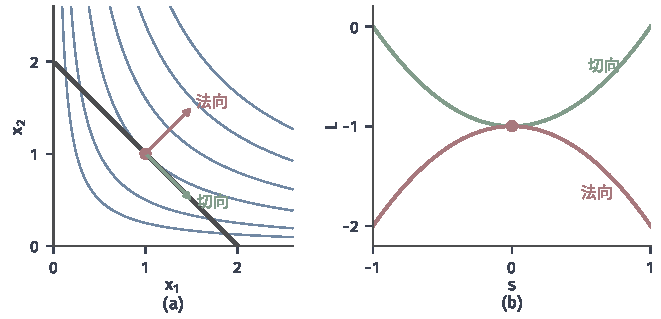
\includegraphics[width=112mm]{figures/05-optimization/06-constrained-optimization/matplotlib/sens-equality-tangent/figure.pdf}
 \caption{切空间上的正定性。(a)~蓝线是$x_1x_2$的等值线，深灰线是约束$x_1+x_2=2$，红点是解，绿色箭头是切方向，红色箭头是法方向。(b)~取$\nu=1$，Lagrange函数沿切方向$(1+s,1-s)$的值是$s^2-1$（绿线），沿法方向$(1+s,1+s)$的值是$-1-s^2$（红线）。}
 \label{fig:sens-equality-tangent}
\end{BookInlineFigure}

Lagrange函数对$\bm{x}$的梯度是
\[
 \nabla_{\bm{x}}\mathcal{L}=(-x_2+\nu\theta,\ -x_1+\nu),
\]
它对$\theta$的偏导数是$(\nu,0)$，而$\partial h/\partial\theta=x_1$。在基准点，这些量都已知，式~\eqref{eq:sens-equality-derivative}成为
\[
 \begin{bmatrix}0&-1&1\\-1&0&1\\1&1&0\end{bmatrix}
 \begin{bmatrix}x_1'\\x_2'\\\nu'\end{bmatrix}
 =-\begin{bmatrix}1\\0\\1\end{bmatrix}.
\]

第二行给出$\nu'=x_1'$，第一行给出$x_2'=x_1'+1$，代入第三行$x_1'+x_2'=-1$，得到
\[
 x_1'=-1,\qquad x_2'=0,\qquad\nu'=-1.
\]
这与显式解在$\theta=1$的导数一致：涨价时第一种投入减少，第二种投入不变。

如果把目标改成$+x_1x_2$，KKT矩阵仍然可逆，隐函数定理仍然给出同样的分支，但切方向的曲率变成$-2$，这条分支上全是约束极大点。可逆只说明方程的解光滑，极小性要靠曲率的符号。

\paragraph{去掉条件会怎样}
先去掉切空间正定性。考虑$\min\tfrac12x_2^2$，约束$x_2-\theta=0$。约束梯度$(0,1)$非零，但切方向$(1,0)$上$\bm{W}=\operatorname{diag}(0,1)$的曲率为零。此时$\bm{K}$的第一行全为零，矩阵奇异。解集是整条直线$\{(s,\theta):s\in\mathbb{R}\}$，“解的导数”没有确定的含义。

再去掉行满秩。考虑$\min x$，约束$x^2-\theta=0$。$\theta>0$时可行集是$\{\pm\sqrt{\theta}\}$，最小点是$x=-\sqrt{\theta}$，导数是$-1/(2\sqrt{\theta})$，$\theta\downarrow0$时趋于$-\infty$。在$\theta=0$处约束梯度$2x$为零，平稳条件$1+2x\nu=0$在$x=0$处没有解，KKT条件本身就不成立。

\subsection{不等式约束极小解}
\label{sec:sens-inequality}

不等式比等式多了一件事：哪些约束起作用，可能随参数改变。本小节的思路是，只要局部上活动约束不变，就把它们当作等式，回到上一小节的情形。

\paragraph{需要的三个条件}
考虑一般问题~\eqref{eq:sens-general-problem}，设$(\bm{x}_0,\bm{\lambda}_0,\bm{\nu}_0)$是$\bm{\theta}_0$处的KKT点，$A=\{i:g_i(\bm{x}_0,\bm{\theta}_0)=0\}$是活动集，$a$是其元素个数。这里用到第~\ref{chap:constrained-optimality}章的三个概念。

\begin{itemize}
 \item \emph{线性无关约束资格}（LICQ）：活动不等式的梯度和全部等式的梯度线性无关。
 \item \emph{严格互补}：每个活动不等式的乘子都严格为正，$\lambda_{0,i}>0$（$i\in A$）。
 \item \emph{二阶充分条件}：$\bm{W}=\nabla^2_{\bm{x}\bm{x}}\mathcal{L}$在临界锥上正定。严格互补成立时，临界锥就是子空间$\ker\bm{J}$，其中$\bm{J}$的行是活动不等式和全部等式的梯度。
\end{itemize}

把活动的不等式改写成等式，定义未知向量$\bm{w}=(\bm{\lambda}_A,\bm{\nu})$，得到一个缩减的方程组
\begin{equation}
 \bm{F}(\bm{x},\bm{w},\bm{\theta})=\begin{bmatrix}\nabla_{\bm{x}}\mathcal{L}\\\bm{g}_A(\bm{x},\bm{\theta})\\\bm{h}(\bm{x},\bm{\theta})\end{bmatrix}=\bm{0}.
 \label{eq:sens-reduced-kkt}
\end{equation}
活动约束的乘子和等式乘子是未知量，不活动约束的乘子取为零，不进入方程。

\begin{theorem}[不等式约束极小解的导数]
\label{thm:sens-inequality}
设$f,g_i,h_j$在$(\bm{x}_0,\bm{\theta}_0)$的邻域内二阶连续可微，$(\bm{x}_0,\bm{\lambda}_0,\bm{\nu}_0)$是KKT点，LICQ、严格互补与二阶充分条件成立。则存在$\bm{\theta}_0$的邻域和唯一的连续可微映射$(\bm{x}(\cdot),\bm{\lambda}(\cdot),\bm{\nu}(\cdot))$，它在基准处经过基准点，邻域内的每一点都是相应问题的KKT点，活动集恒为$A$，$\bm{x}(\bm{\theta})$是严格局部极小点。导数$\bm{D}_{\bm{x}}$、$\bm{D}_{\bm{w}}$满足
\begin{equation}
 \begin{bmatrix}\bm{W}&\bm{J}^{\top}\\\bm{J}&\bm{0}\end{bmatrix}
 \begin{bmatrix}\bm{D}_{\bm{x}}\\\bm{D}_{\bm{w}}\end{bmatrix}
 =-\begin{bmatrix}\nabla^2_{\bm{x}\bm{\theta}}\mathcal{L}\\\bm{D}_{\bm{\theta}}(\bm{g}_A,\bm{h})\end{bmatrix}.
 \label{eq:sens-inequality-derivative}
\end{equation}
\end{theorem}

\begin{proof}
LICQ就是$\bm{J}$行满秩，严格互补使二阶充分条件成为$\bm{W}$在$\ker\bm{J}$上正定。由引理~\ref{lem:sens-kkt-invertible}，矩阵$\bm{K}$可逆，隐函数定理给出式~\eqref{eq:sens-reduced-kkt}的连续可微解$(\bm{x}(\bm{\theta}),\bm{w}(\bm{\theta}))$，求导得到式~\eqref{eq:sens-inequality-derivative}。

下面验证这个解确实是完整问题的KKT点。不活动约束满足$g_i(\bm{x}_0,\bm{\theta}_0)<0$，由连续性，附近仍有$g_i(\bm{x}(\bm{\theta}),\bm{\theta})<0$，把它们的乘子取为零。活动约束的乘子满足$\lambda_{0,i}>0$，由连续性，附近仍有$\lambda_i(\bm{\theta})>0$。于是可行性、乘子符号和互补松弛全部成立，活动集仍是$A$，且严格互补仍成立。

与定理~\ref{thm:sens-equality}相同的连续性论证说明，$\bm{J}$行满秩和$\ker\bm{J}$上的正定性在附近保持，二阶充分条件推出$\bm{x}(\bm{\theta})$是严格局部极小点。

最后看唯一性。若完整问题另有KKT点靠近基准点，不活动约束仍严格满足，其乘子必为零；活动约束的乘子靠近正数$\lambda_{0,i}$，也为正，由互补松弛这些约束取等号。这个点于是满足式~\eqref{eq:sens-reduced-kkt}，由隐函数定理的唯一性，它就在分支上。
\end{proof}

图~\ref{fig:sens-kkt-block}画出式~\eqref{eq:sens-inequality-derivative}的结构。系数矩阵只由基准点的量决定，$q$个参数对应$q$列右端。

\begin{BookInlineFigure}
 \centering
 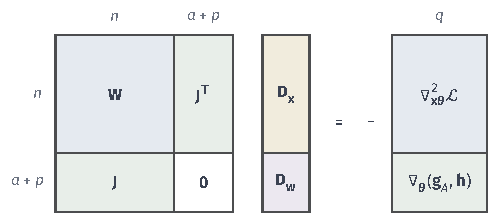
\includegraphics[width=83mm]{figures/05-optimization/06-constrained-optimization/tikz/sens-kkt-block/figure.pdf}
 \caption{式~\eqref{eq:sens-inequality-derivative}的分块结构。系数矩阵的阶数是$n+a+p$，其中$a$是活动不等式个数，$p$是等式个数。$\bm{D}_{\bm{x}}$与$\bm{D}_{\bm{w}}$是待求的Jacobian矩阵，右端共$q$列，每列对应一个参数。不活动约束不出现在这个方程组中。}
 \label{fig:sens-kkt-block}
\end{BookInlineFigure}

\paragraph{预算例的两个活动集}
取$\tau=2$。活动集是$\{1\}$，方程组与第~\ref{sec:sens-equality}节的预算线例子完全相同，因为只有预算在起作用：
\[
 x_1'=x_2'=\frac12,\qquad\lambda_1'=-\frac12.
\]

取$\tau=0.5$。解是$(0.5,0)$，乘子是$\lambda_1=3/2$，$\lambda_3=1/2$，活动集是$\{1,3\}$。此时$\bm{W}=\bm{I}$，活动约束的梯度组成
\[
 \bm{J}=\begin{bmatrix}1&1\\0&-1\end{bmatrix},\qquad
 \frac{\partial}{\partial\tau}\begin{bmatrix}g_1\\g_3\end{bmatrix}=\begin{bmatrix}-1\\0\end{bmatrix}.
\]

$\ker\bm{J}$只含零向量，切空间的正定性自动成立。式~\eqref{eq:sens-inequality-derivative}的四行分别是
\[
 x_1'+\lambda_1'=0,\quad
 x_2'+\lambda_1'-\lambda_3'=0,\quad
 x_1'+x_2'=1,\quad
 -x_2'=0.
\]
依次解出
\[
 x_2'=0,\qquad x_1'=1,\qquad\lambda_1'=-1,\qquad\lambda_3'=-1.
\]
这时增加的预算全部给第一种投入，因为$x_2$被边界挡在零上。

\paragraph{严格互补和余量给出窗口}
严格互补与不活动约束的严格余量在定理中起同一种作用：它们留出一段余地，让参数小幅变化时符号条件不被破坏。这段余地有多大，可以用导数估计。

在$\tau=2$处，三个要保持为正的量分别是不活动约束的余量$x_1$、$x_2$和活动约束的乘子$\lambda_1$。沿分支它们是
\[
 x_1=\frac{\tau+1}{2},\qquad
 x_2=\frac{\tau-1}{2},\qquad
 \lambda_1=\frac{3-\tau}{2}.
\]

第一个到达零的是$x_2$（$\tau=1$）和$\lambda_1$（$\tau=3$），分支的有效窗口是$1<\tau<3$，见图~\ref{fig:sens-margins}。窗口的一端是不活动约束变成活动，另一端是活动约束不再起作用。

\begin{BookInlineFigure}
 \centering
 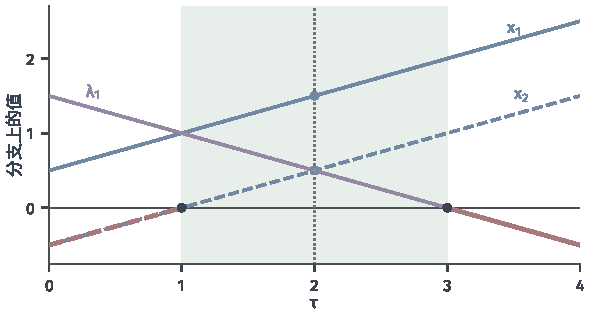
\includegraphics[width=100mm]{figures/05-optimization/06-constrained-optimization/matplotlib/sens-margins/figure.pdf}
 \caption{活动集$\{1\}$的分支把公式延拓到窗口之外。蓝色实线与虚线是不活动约束的余量$x_1$、$x_2$，紫线是乘子$\lambda_1$，绿色区域是三者都为正的窗口$1<\tau<3$。红色部分是符号条件被破坏之处：$\tau<1$时$x_2<0$不可行，$\tau>3$时$\lambda_1<0$不满足KKT条件。}
 \label{fig:sens-margins}
\end{BookInlineFigure}

\paragraph{这些条件只是充分的}
定理的三个条件对解可微是充分条件，下面三个例子逐一说明它们都不是必要的。

严格互补不必要：考虑$\min\tfrac12(x-\theta^2)^2$，约束$x\geq0$。解是$x=\theta^2$，处处可微。而在$\theta=0$处，约束活动且乘子为零，严格互补不成立。

LICQ不必要：约束写两遍$\theta-x\leq0$，目标取$\min x$。解$x=\theta$处处可微，两条活动约束的梯度相同，LICQ不成立，乘子也不唯一。

二阶充分条件不必要：考虑$\min x^4/4-\theta^3x$，驻点方程$x^3=\theta^3$给出$x=\theta$，处处可微。而在$\theta=0$处Hessian等于零。

反过来，这些条件被破坏时，导数常常确实失效，下一节拆开具体的失效方式。定理不能用来断言“条件不成立，所以不可微”。
